\documentclass[5pt]{article}
\usepackage{mathptmx,amsmath}
\usepackage{pdfslide2,pause}
\usepackage{eurosym}
\usepackage[portuguese,english]{babel}
%\usepackage{kerkis}
\usepackage{colortbl} % used to highlight row or columns of tables. http://www.tug.org/pracjourn/2007-1/mori/mori.pdf
\usepackage[small]{caption} % more option on http://www.dd.chalmers.se/latex/Docs/PDF/caption.pdf
\usepackage[tight,scriptsize]{subfigure}
\usepackage{lastpage}
\usepackage{chngcntr}
\usepackage[absolute,overlay]{textpos}
\usepackage{tabto}
\usepackage{animate}
%\usepackage{listings}
\captionsetup{labelformat=empty,skip=-0.8cm}

%%%% Diamantino %%%%
% As minhas packages
\usepackage[utf8]{inputenc}
\usepackage{braket}

%\lstset{
%    language=Matlab,                % choose the language of the code
%    basicstyle=\ttfamily\tiny,      % the size of the fonts that are used for the code
%    numbers=none,                   % where to put the line-numbers
%    numberstyle=\tiny,              % the size of the fonts that are used for the line-numbers
%    stepnumber=1,                   % the step between two line-numbers. If it's 1 each line will be numbered
%    numbersep=5pt,                  % how far the line-numbers are from the code
%    backgroundcolor=\color{white},  % choose the background color. You must add \usepackage{color}
%    showspaces=false,               % show spaces adding particular underscores
%    showstringspaces=false,         % underline spaces within strings
%    showtabs=false,                 % show tabs within strings adding particular underscores
%    tab=\rightarrowfill,
%    frame=none,	                 % adds a frame around the code
%    tabsize=2,	                     % sets default tabsize to 2 spaces
%    captionpos=b,                   % sets the caption-position to bottom
%    breaklines=true,                % sets automatic line breaking
%    breakatwhitespace=false,        % sets if automatic breaks should only happen at whitespace
%    title=\lstname,                 % show the filename of files included with \lstinputlisting; also try caption instead of title
%    escapeinside={\%*}{*)},          % if you want to add a comment within your code
%    morekeywords={ifftshift,fftshift},
%    keywordstyle=\bfseries\color[rgb]{0,0,0.3},
%    commentstyle=\color[rgb]{0.133,0.5,0.133}
%}
%\lstset{
%    emph={function,end,for,if,while},
%    emphstyle=\bfseries\color[rgb]{0.6,0,0},
%}

\definecolor{itblue}{rgb}{0.0,0.0,0.5}
\definecolor{itred}{rgb}{0.82,0.18,0.24}
\newcommand{\pageNum}{
    \begin{picture}(0,0)(0,0)
        \put(-15,-390){
            \begin{minipage}{1.8cm}
            \end{minipage}
        }
    \end{picture}
}
\newcommand{\cb}[1]{{\color{itblue} #1}}%
\newcommand{\cred}[1]{{\color{itred} #1}}%
\newcommand{\bb}[1]{{\textbf{\color{itblue} #1}}}%
\newcommand{\br}[1]{{\textbf{\color{itred} #1}}}%
\renewcommand{\labelitemi}{\textcolor{itred}{\normalsize $\bullet$}}
\renewcommand{\labelitemii}{\textcolor{itblue}{$\bullet$}}
\newcommand{\mysection}[1]{\section*{\pageNum\color{itred}\sffamily #1}\vspace*{0.5cm}\overlay{./figures/it_1.png}\sffamily}%
\newcommand{\ITfootnote}[1]{\hspace{1.8cm}\begin{minipage}{13cm}\tiny{#1}\end{minipage}}
\newcommand{\edfaGain}{$G=\exp\left(\frac{\alpha}{2}L_{span}\right)$}
\newenvironment{reference}{
    \begin{textblock*}{0.7\textwidth}(32mm,137mm)\tiny\noindent\bgroup\color{black}
}
{
    \egroup\end{textblock*}
}


\graphicspath{{./Figures/}}
\pagestyle{title}

\hyphenpenalty=50000
\tolerance=10000

\setlength{\textheight}{1.5\textheight}

%%%%%%%%%%%%%%%%%%%%%%%%%%%%%%%%%%%%%%%%%%%%%%%%%%%%%%%%%%%%%%%%%%%%%%%%%%%%%%%%
%%%%%%%%%%%%%%%%%%%%%%%%%%%%%%%%%%%%%%%%%%%%%%%%%%%%%%%%%%%%%%%%%%%%%%%%%%%%%%%%

\begin{document}

%*******************************************************************************
%                                          SLIDE
%*******************************************************************************
\pagenumbering{roman}
\begin{titlepage}  \overlay{./figures/it_0.png}

\color{itblue} \sffamily \noindent \small
\hspace*{1cm}  Universidade de Aveiro\\
\hspace*{1cm}  2017-2018\\ %Lisboa, 14th of February, 2013\\

\vspace*{1cm}
\begin{center}
    \color{black} \sffamily \noindent \Large
    \br{Real-time shot-noise measurement\\}
\end{center}
\vspace{6mm}
\begin{center}
    \color{black}
    \textbf{Diamantino Silva\\}
    {(diamantinosilva@ua.pt)}
\end{center}

\vspace{0.0mm}
\scriptsize
\begin{center}
Department of Electronics, Telecommunications and Informatics,\\
University of Aveiro, Aveiro, Portugal\\
Instituto de Telecomunicações, Aveiro, Portugal\\
\end{center}

\vspace{1.0cm}
\hfill \tiny \copyright 2005, it - instituto de telecomunicações\hfill

\end{titlepage}


\renewcommand{\headsep}{-25pt}
\pagenumbering{arabic}



%-------------------------------------------------------------------------------
%----------------------------------- SLIDE -------------------------------------
\mysection{Real-time quantum noise measurement}\large
\vspace{0cm}

\noindent

\vspace{1cm}

\begin{center}
Analysis of the paper
\end{center}

\vspace{1em}

\begin{center}
\textbf{Practical performance of real-time shot-noise measurement in continuous-variable quantum key distribution}
\end{center}

\begin{center}
Tao Wang, Peng Huang, Yingming Zhou, Weiqi Liu, Guihua Zeng
\end{center}

\begin{center}
2017
\end{center}

%-------------------------------------------------------------------------------
%----------------------------------- SLIDE -------------------------------------
%\mysection{CVQKD}\large
%\vspace{0cm}
%
%QKD is...\\
%
%QKD is a quantum information technology primitive which allows two distant parties, Alice and Bob, to establish a secret key out of communications through an untrusted physical channel and a public authenticated channel. It's advantage over classical cryptography primitives is that the produced keys are secure in the information-theoretic sense even against an eavesdropper...\\
%\\
%This study focus on the Gaussian modulated coherent state (GMCS) scheme.\\


%-------------------------------------------------------------------------------
%----------------------------------- SLIDE -------------------------------------
\mysection{RTSNM - the problem}\large
\vspace{0cm}


\noindent
For any QKD system, some statistics about the transmitted data are used to evaluate the amount of information that may be in possession of an attacker.\\
\\
The estimation of the eavesdropper information depends on the \textbf{excess noise} which is the difference between the observed noise and the shot noise, and also on the \textbf{observed correlation} between the emitter and the receiver.\\
\\
The historical method to estimate the shot noise is to calibrate once and for all the slope of the local oscillator to shot noise linear relation on the homodyne detection, and then to measure in real time the power of the local oscillator.\\
\\
It was shown that this relationship is \textbf{prone to change over time}, especially under the influence of an attacker.\\

%-------------------------------------------------------------------------------
%----------------------------------- SLIDE -------------------------------------
\mysection{RTSNM - a solution}\large
\vspace{0cm}

\noindent
In order to defend practical attacks, real-time monitoring technologies are extensively adopted to prevent both attack and signal disturbance.\\
\\
RTSNM is proposed as a "procedure for preventing the eavesdropper exploiting the practical security loopholes" of CVQKD, such as fluctuations of local oscillator intensity.\\



%-------------------------------------------------------------------------------
%----------------------------------- SLIDE -------------------------------------
\mysection{CVQKD}\large
\vspace{0cm}

\noindent
Alice generates two random numbers $X_A$ and $P_A$ from gaussian distributions, both with mean $0$ and variance $V_A$, and prepares a coherent state $\ket{X_A + i P_A}$, which sends to Bob.\\
Bob receives polarized-multiplexed pulses, in which the signal (S) is in the $X$ polarization and the local oscillator (LO) is in the $Y$ polarization.
A phase modulator randomly generates a $\Psi$ ($0$ or $\pi/2$) phase shift to measure either $x$ or $p$. Then, the LO and S interfere in a homodyne detector, which output intensity is proportional to the modulated quadratures.




%-------------------------------------------------------------------------------
%----------------------------------- SLIDE -------------------------------------
\mysection{RTSNM - Implementation}\large
\vspace{0cm}

\begin{figure}[h!]
	\centering
	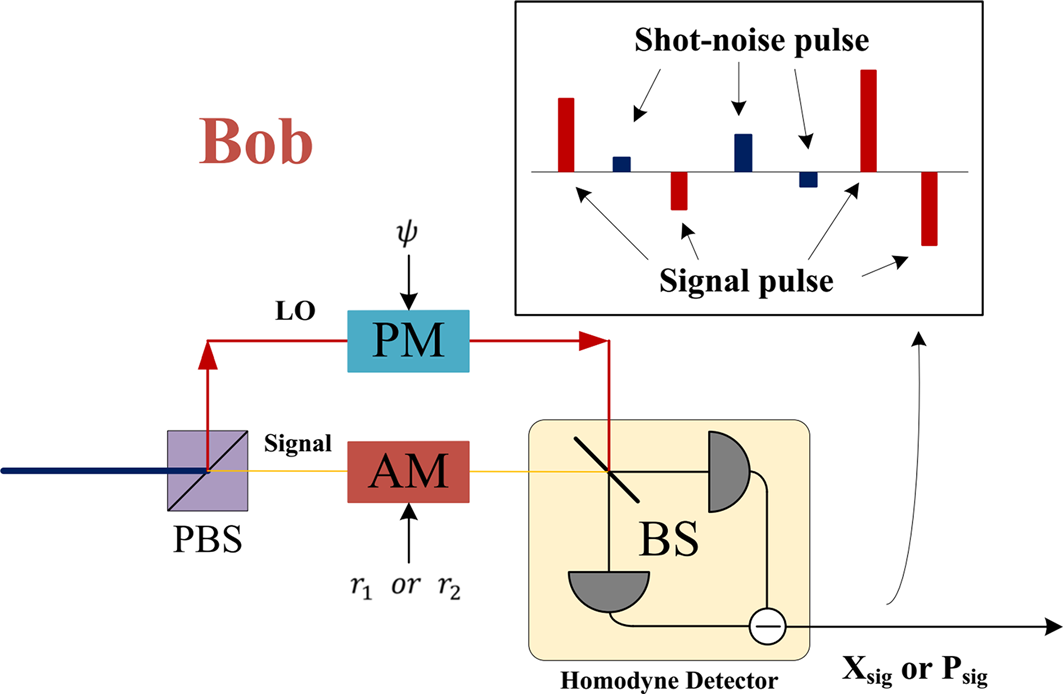
\includegraphics[width=0.5\textwidth]{figures/RTSNM-fig1.png}
\end{figure}

\vspace{1em}
\noindent
The difference to the standard CVQKD protocol resides on the amplitude modulator (AM) introduced in Bob's signal path. This will allow to choose between two extintion ratios ($r_1=1$ or $r_2=0$), of the AM to measure the signal pulse or the shot-noise pulse. 


%-------------------------------------------------------------------------------
%----------------------------------- SLIDE -------------------------------------
\mysection{RTSNM - Implementation}\large
\vspace{0cm}

After a quantum transmission, Alice and Bob share two correlated vectors $P=\{(x_i, y_i)|i=1,2,...N\}$, where $N$ is the total number of received data when the extintion ratio was $r_1$. 
Meanwhile, Bob also acquires a single vector $Q=\{(y_{0i})|i=1,2,...,N'\}$, where $N'$ is the total number when the ratio ir $r_2$.

%From these pairs of correlated pairs, some xxx quantity is chosen to estimate the parameters of the channel??\\

%Os parametros sao estimados e se eles forem compativeis com uma chave secreta positiva, entao podem aceitar a chave, senao, cancelam o protocolo.


%-------------------------------------------------------------------------------
%----------------------------------- SLIDE -------------------------------------
\mysection{RTSNM - Channel model}\large
\vspace{0cm}

\noindent
The quantum channel of CVQKD is a normal linear model with the following relations between Alice and Bob
$$
	y = tx + z, \quad y_0 = z_0
$$
in which $t=\sqrt{\eta T}$, $z$ is the total noise term and $z_0$ is the partial noisel, both gaussian random variables.\\
%
\begin{center}
	\begin{tabular}{l l}
		$\eta$			& efficiency of the homodyne detection\\
		$T$				& transmission of the quantum channel\\
		$N_0$			& variance of shot noise\\
		$\varepsilon$	& excess noise (in SN units)\\
		$V_{el}$		& detector's electronic noise\\
	\end{tabular}
\end{center}




%-------------------------------------------------------------------------------
%----------------------------------- SLIDE -------------------------------------
\mysection{RTSNM - Channel Model}\large
\vspace{0cm}

\begin{center}
	\begin{tabular}{c c c}
		\hline
		\textbf{Variable}	& \textbf{Mean}		& \textbf{Variance}\\
		\hline
		$x$					& 0					& $V_A$\\
		$y$					& 0					& $\eta T V_A + \eta T \varepsilon N_0 + N_0 + V_{el}$\\
		$z$					& 0					& $\eta T \varepsilon N_0 + N_0 + V_{el}$\\
		$y_0$				& 0					& $N_0 + V_{el}$\\
		$z_0$				& 0					& $N_0 + V_{el}$\\
		\hline
	\end{tabular}
\end{center}

\vspace{1em}

\begin{center}
	\begin{tabular}{c p{12cm}}
		\hline
		\textbf{Variance term}		& \textbf{Description}\\	
		\hline
		$V_A$						& \small{Variance of the parameters of the coherent state}\\ 
		$N_0$						& \small{Shot noise variance}\\
		$V_{el}$					& \small{Detector's electronic noise}\\
		$\eta T V_A$				& \small{$V_A$ after the channel transmission and detection}\\ 
		$\eta T \varepsilon N_0$	& \small{"The noise in Bob's state in excess compared to the shot noise"?}\\
		\hline
	\end{tabular}
\end{center}




%-------------------------------------------------------------------------------
%----------------------------------- SLIDE -------------------------------------
\mysection{RTSNM - Estimators}\large
\vspace{0cm}
Parameteres that need to be estimated
\begin{center}
	\begin{tabular}{c l}
		\hline
		\textbf{Parameter}	& \textbf{Description}\\	
		\hline
		$T$					& transmission of the quantum channel\\
		$N_0$				& variance of shot noise\\
		$\varepsilon$		& excess noise (in SN units)\\
		\hline
	\end{tabular}
\end{center}
%
\vspace{1em}
From the $P$ vector, $m$ pairs ($m<N$) of correlated data are randomly selected to use in the parameter estimation.
Bob uses $m'=N'$ data samples from the vector $Q$ to perform the shot-noise estimation procedure.\\
%
\begin{center}
	\begin{tabular}{l l}
		Correlation of Alice and Bob values & $\hat{t} = \frac{\sum_{i=1}^m x_i y_i}{\sum_{i=1}^m x_i^2} $\\
		Estimator of the variance of $z$ & $\hat{\sigma}^2 = \frac{1}{m} \sum_{i=1}^m ( y_i - \hat{t} x_i)^2$\\
		Estimator of the variance of $z_0$ & $\hat{\sigma_0}^2 = \frac{1}{m'} \sum_{i=1}^{m'} ( y_{0i})^2$\\
	\end{tabular}
\end{center}




%-------------------------------------------------------------------------------
%----------------------------------- SLIDE -------------------------------------
\mysection{RTSNM - Estimators}\large

\vspace{1em}

The real values of the threes quantities should be in the interval
$$
	t \in \left[ \hat{t} - \Delta t, \hat{t} + \Delta t \right], \quad
$$
$$
	\sigma^2 \in \left[ \hat{\sigma}^2 - \Delta \sigma^2, \hat{\sigma}^2 + \Delta \sigma^2  \right], \quad
	\sigma_0^2 \in \left[ \hat{\sigma_0}^2 - \Delta \sigma_0^2, \hat{\sigma_0}^2 + \Delta \sigma_0^2  \right]
$$

The estimators should obtain the most pessimist estimation for the quantity of information obtained by an eavesdropper.
We end up with the following estimatives
$$
T_{min} = (\hat{t} - \Delta t)^2 / \eta, \quad
\varepsilon_{max} = \frac
{\left(\hat{\sigma}^2 + \Delta \hat{\sigma}^2 - \hat{\sigma_0}^2 \right)}
{\hat{t}^2\left(\hat{\sigma_0}^2 - V_{el}\right)}
$$
in which
$$
\Delta t = z_{\epsilon_{PE}/2}\sqrt{\frac{\hat{\sigma}^2}{mV_A}}, \quad
\Delta \sigma^2 = z_{\epsilon_{PE}/2} \frac{\hat{\sigma}^2 \sqrt{2}}{\sqrt{m}}, \quad
\Delta \sigma_0^2 = z_{\epsilon_{PE}/2} \frac{\hat{\sigma_0}^2 \sqrt{2}}{\sqrt{m'}}
$$




%-------------------------------------------------------------------------------
%----------------------------------- SLIDE -------------------------------------
\mysection{RTSNM - Problems of the Solution}\large
\vspace{0cm}

\noindent
\textbf{Small size effects}\\
Given the size of the blocks (N) and the size of the analysed pulses for estimating the parameters, noise is introduced in the system.\\
%Nao propriemente ruido, mas sim erros de estimacao e menos seguranca.
\\
\textbf{Imperfect amplitude modulation}\\
Because there are no perfect modulators,..\\
\\
\\
"In short, using this RTSNM scheme, although the pratical security and stability of the system are improved, we may sacrifice the transmission distance and the final key rate."




%-------------------------------------------------------------------------------
%----------------------------------- SLIDE -------------------------------------
\mysection{} \sffamily
\vspace{-10mm}
\large\centerline{E-mail: diamantinosilva@ua.pt}


\end{document}


% PROTOTIPO DE UM SLIDE

%%-------------------------------------------------------------------------------
%%----------------------------------- SLIDE -------------------------------------
%\mysection{RTSNM - Problems of the Solution}\large
%\vspace{0cm}
%

